%%%%%%%%%%%%%%%%%%%%%%%%%%%%%%%%%%%%%%%%%%%%%%%%%%%%%%%
% Math 3250 Combinatorics, University of Connecticut
%%%%%%%%%%%%%%%%%%%%%%%%%%%%%%%%%%%%%%%%%%%%%%%%%%%%%%%

% Anything after a percent sign is a comment.

% Necessary first line. \documentclass defines the type of document and some options (for example, try changing 12pt to 10pt.
\documentclass[12pt]{amsart}
\usepackage{enumerate} % to be able to enumerate a list using non-numbers
\usepackage{tikz}


% The part of the tex file between the \documentclass and \begin{document} line is called the preamble.  Things having to do with setting up the document are done in the preamble.  You will not need to mess with it for now, except to change your name and the title of your document. 
% After adding your name next to author, head down to where it says "Start here"

\title{Math3250 Combinatorics Week3 Problem Set}
\author{your preferred first and last name}
\date{}
\begin{document}

\maketitle

% --------------------------------------------------------
%                         Start here
% --------------------------------------------------------

\noindent Credit: Write down everyone who helped you, including classmates who contributed to your thought process (either through sharing insights or through being a sounding board). Write down Bona's textbook and other written sources you used as well.

\subsection*{Instruction}
%Submit only Problems using  \LaTeX. 
The exact problems will be announced on Monday during class. 
Please send me an invite via Overleaf. %by entering my UConn email address.

Note: For your convenience, please use the SAMPLE SOLUTION below as a template for typing up an induction proof. 

If you are not sure how to do something, please post on Piazza or come to office hour.


\section*{Sample Solution}
Let the sequence $\{ a_n\}$ be defined by the relations $a_0=1$, and let
\[
a_{n+1} = 2(a_0 + a_1 + \dots + a_n) 
\]
for $n \geq 0$. 
Compute the first few values of $a_n$, then conjecture an explicit formula for $a_n$, and then prove the formula using induction.
\begin{proof}[Solution and proof]
We claim that $a_n = 2 \cdot 3^{n-1}$ for $n \geq 1$. We prove this by strong induction on $n$.
Since $2(a_0)=2(1)=2\cdot 3^{1-1}$, the initial case (for $n=1$) is verified.  
Now let us assume that the statement is true for all positive integers that are less than or equal to $n$. Then, we have
\begin{align*}
    a_{n+1} &= 2(a_0 + a_1 + a_2 + \dots + a_n) ~ \text{ by the recurrence relation}\\
    &= 2 a_0 + 2 (a_1 + a_2 + \dots +  a_n)\\
    &= 2 + 2(2 \cdot 1 + 2 \cdot 3 + \dots + 2 \cdot 3^{n-1}) ~ \text{ by the induction hypothesis}\\
     &= 2 + 4 ( 1 +  3 + \dots +  3^{n-1})\\
     &= 2 + 4 \left( \frac{3^n - 1}{2}  \right) ~ \text{ since the series is a geometric series} \\
     &= 2 + 2 (3^n - 1) \\
     &= 2 \cdot 3^n.
\end{align*}
This proves that our explicit formula is correct for $n+1$, and the proof is complete.
\end{proof}


\section{Recurrence relation}
Let the sequence $\{ a_n\}$ be defined by the relations $a_0=1$, and 
\[
a_n = 3(a_0 + a_1 + \dots + a_{n-1}) + 1
\]
for $n>0$. 
Compute the first few values of $a_n$, then conjecture an explicit formula for $a_n$, and then prove the formula using induction.

%Click here for a hint: Use Sec 2.2 Strong Induction. Copy and paste the sample solution typed above.  Follow Example 2.5 and Example 2.6 in the book and also the sample solution typed above.

\begin{proof}
Insert proof
\end{proof}

\section{polygon}
Prove (using induction) that the sum of the angles of a convex $n$-gon is $(n-2)180$ degrees.

Note: You may use the fact (possibly proven in your geometry class) about the sum of angles of a convex triangle without proof.
\begin{proof}
Insert proof
\end{proof}

\section{Divisible by eleven}
Prove that a positive integer with digits $a_1, a_2, \dots, a_n$ is divisible by $11$ if and only if $a_1 - a_2 + a_3 - \dots + (-1)^{n-1} a_n$ is divisible by $11$

%Click here for a hint: Use Section 2.2 Strong Induction. The initial step is to verify the statement for the integers $1$, $2$, $\dots$, $98$, $99$ with fewer than $3$ digits.
\begin{proof}
Insert proof
\end{proof}


\section{Divisible by three}
Prove that a positive integer is divisible by $3$ if and only if the sum of its digits is divisible by $3$.

%Click here for a hint: Use Section 2.2 Strong Induction. 
\begin{proof}
Insert proof
\end{proof}


\section{Squares}
We start with one square piece of paper 
\begin{tikzpicture}[scale=2]
\draw(0,0) grid (1,1);
\end{tikzpicture}.

We then cut this square paper into four smaller squares
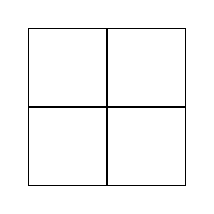
\begin{tikzpicture}
\draw(0,0) grid (2,2);
\end{tikzpicture}.

Then cut one of the obtained small squares into four smaller squares, so that we get $7$ squares 
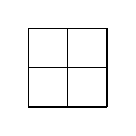
\begin{tikzpicture}[scale=0.5]
\draw(0,0) grid (2,2);
\end{tikzpicture} \hspace {-1cm}
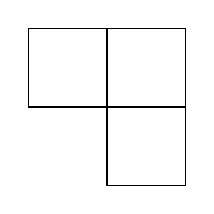
\begin{tikzpicture}
\draw(1,1) grid (0,0);
\draw(1,1) grid (2,0);
\draw(1,0) grid (2,-1);
\end{tikzpicture}, 
and so on.

Let $a_n$ be the number of squares we have after the $n$-th time that we perform this cutting operation. 
Compute the first few values of $a_n$ (beyond $n=1$ and $n=2$ given above), then conjecture an explicit formula for $a_n$, and then prove the formula using induction.
\begin{proof}
Insert proof
\end{proof}



\section{6 digit numbers}
\begin{enumerate}[a)]
    \item  How many $6$ digit numbers are there (leading zeros, e.g. $001223$ not allowed)? 
    \item How many of these are even? 
    \item How many 6 digit numbers are there with exactly one 7? 
    \item How many 6 digit numbers are there that are the same forward and backwards (e.g., $890098$)?
\end{enumerate}

\begin{proof}
Insert answers and explanations
\end{proof}



\section{BAA, ABA, AAB}
How many 3 digit positive integers contain two (but not three) digits?


\section{Sandwich shop} 
A sandwich shop has $4$ protein options. 
It also has $6$ veggies: lettuce, sprouts, carrots, onion, tomato and pickles. It carries $5$ sauces: mustard, catsup, mayo, sirachi, and vinegar. How many sandwiches can be made from one protein, one veggie and AT MOST one sauce?
\begin{proof}
Insert answer and a brief reasoning.
\end{proof}



\section{Connecticut}
Compute the number of ways to create a  list (of size $11$) of the letters of the word CONNECTICUT. 
\begin{proof}
Insert answer and a brief reasoning.
\end{proof}

\section{Alternating parity}
\begin{enumerate}[a)]
    \item Warm-up: In how many ways can the elements of $[3]$ be permuted so that the sum of every two consecutive elements in the permutation is odd? 
    In how many ways can the elements of $[4]$ be permuted so that the sum of every two consecutive elements in the permutation is odd?

    \item (Optional) Compute this for $[5]$ as well.

    \item In how many ways can the elements of $[n]$ be permuted so that the sum of every two consecutive elements in the permutation is odd?
\end{enumerate}



\section{Write Your Own Problem}\label{sec:write_your_own}
Please write your own problem and solve it using theorems or concepts from Section 2.1-2.2 or Section 3.1 of Bona.
(Student's problems may be chosen for future exams' questions). You may test the difficulty level of your problem by sharing it with a classmate. 

\section{Miscellaneous}
\begin{enumerate}[i.]
    \item Share your work (at least one problem) and thought process with at least one classmate. Ask them to share their thought process as well. Write down their names and briefly summarize your interactions. A virtual discussion via Piazza or email is fine if you don't have time to interact in person. 
    \item Approximately how much time did you spend on this homework?
\end{enumerate}

\end{document}
